%% Exercice 1

%\ExoSpecs{\TTBF{CalculTVA.sh}}{\TTBF{\RenduDir/src/exo1/}}{750}{640}{\TTBF{write}}
\ExoSpecsCustom{\TTBF{bt\_basics.c}}{\TTBF{\RenduDir/src/}}{750}{640}{Fonctions autorisées}{\TTBF{malloc(3)}, \TTBF{free(3)}, \TTBF{printf(3)}}

\vspace*{0.7cm}

\noindent \ExoObjectif{Le but de l'exercice est d'implémenter les outils essentiels aux abres binaires.}

\bigskip

%\noindent Les fonctions demandées dans cet exercice devront se trouver dans une bibliothèque nommée \TTBF{libmystack}.
%Après un appel à la commande \texttt{make} à la racine du projet, il faut que votre chaîne de compilation produise à la racine de votre projet une version statique de la bibliothèque (qui se nommera \TTBF{libmystack.a}) ainsi qu'une version dynamique de la bibliothèque (qui se nommera \TTBF{libmystack.so}).
%
%\bigskip

\noindent Vous devez écrire plusieurs fonctions permettant de construire, parcourir, et vider des arbres binaires en ajoutant des nœuds.
Un fichier \TTBF{bt\_basics.h} contenant toutes les fonctions exportables à implémenter vous est fourni en annexe.
%Vous devez déclarer une structure \TTBF{bt\_p} et l'ajouter dans \TTBF{bt\_basics.h}.
%%N'oubliez pas de déclarer également une structure qui contiendra les éléments de la liste chaînée.
%%Pour les premières étapes, vous devrez implémenter une version simplifiée de la pile qui ne prend en charge que des entiers positifs.
%Cette structure devra prendre en charge la représentation des arbres sous forme de pointeurs, et chaque nœud devra disposer d'un champ \textit{key} sous forme d'entier, d'un champ \textit{elt} sous forme de pointeur générique, et d'un champ \textit{len\_elt} sous forme d'entier (représentant la taille de l'élément).
La structure \TTBF{bt\_p} est déjà déclarée dedans.
Cette structure prend en charge la représentation des arbres sous forme de pointeurs grâce aux champs \textit{lc} (pointeur vers le fils gauche) et \textit{rc} (pointeur vers le fils droit).
Chaque nœud dispose également d'un champ \textit{key} contenant la clé identifiant l'élément stocké, d'un champ \textit{elt} pointant vers l'élément stocké, et d'un champ \textit{len\_elt} représentant la taille de l'élément.

\smallskip

\noindent Vous aurez probablement besoin d'au moins une file.
Vous pouvez ajouter deux fichiers supplémentaires \TTBF{.c} et \TTBF{.h} pour y implémenter votre file et ainsi appeler ces fonctions.

%\noindent Conceptuellement, les fonctions manipulant des piles de type \TTBF{stack\_ll*} devront pouvoir gérer ces 3 cas :

%\bigskip

%\begin{center}
%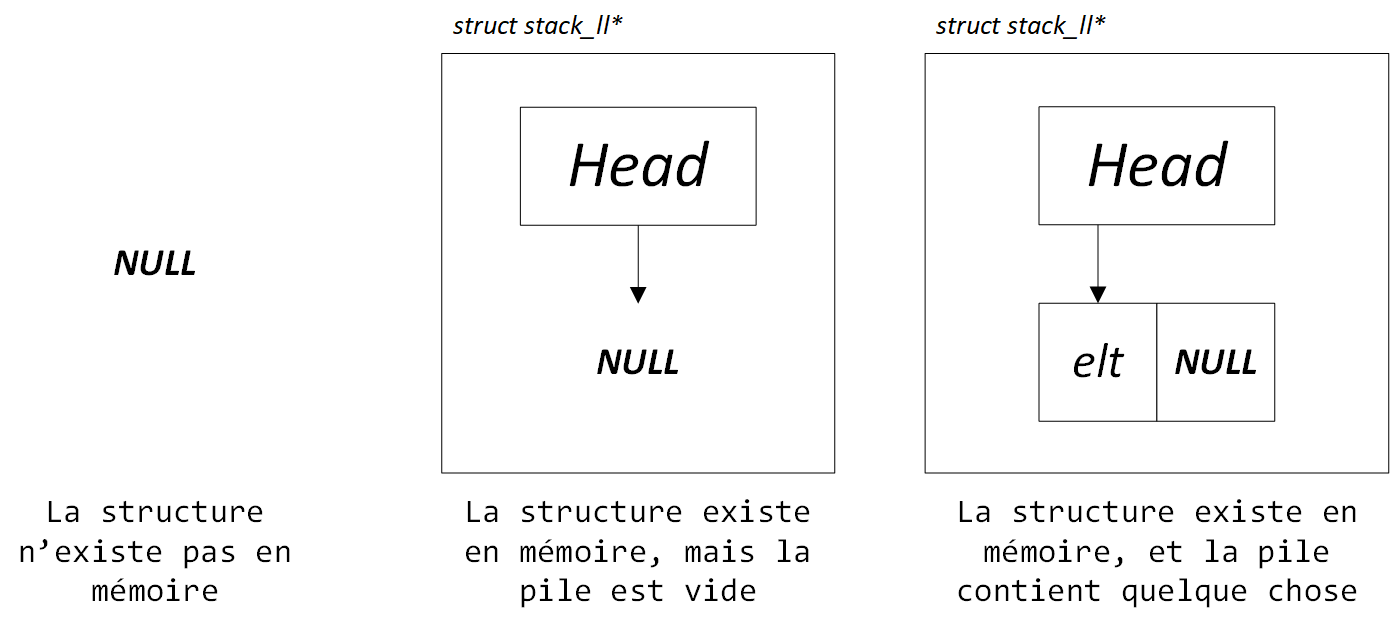
\includegraphics[scale=0.85]{Cours/Piles_Implementation_LL.png}
%\end{center}

\bigskip
%\newpage

\noindent Vous devez implémenter les fonctions suivantes :

\bigskip
%\medskip

\lstset{language=C}
%\begin{lstlisting}[frame=single,title={Liste des fonctions pour une pile avec liste chaînée}]
\begin{lstlisting}[frame=single]
bt_p *create_bt_p(int key,
                  int elt_size,
                  void *elt,
                  bt_p *left_child,
                  bt_p *right_child);
int get_key_bt_p(bt_p *node);
int get_elt_size_bt_p(bt_p *node);
void *get_elt_bt_p(bt_p *node);

int deepness_node_bt_p(bt_p *node, bt_p *T);
int size_bt_p(bt_p *T);
int height_bt_p(bt_p *T);

void print_dfs_preorder_bt_p(bt_p *T);
void print_dfs_inorder_bt_p(bt_p *T);
void print_dfs_postorder_bt_p(bt_p *T);

void print_hierarchical_bt_p(bt_p *T);
int hierarchical_number_bt_p(bt_p *T, int key);

int clear_bt_p(bt_p *T);
\end{lstlisting}


\subsubsection*{\TTBF{bt\_p *create\_bt\_p(int key, int elt\_size, void *elt, bt\_p *left\_child, bt\_p *right\_child)}}

\noindent Cette fonction crée un nœud en remplissant ses différents champs ainsi qu'en indiquant les adresses de ses fils gauche et droit.
En cas d'erreur (pas assez de mémoire), cette fonction doit renvoyer un pointeur \TTBF{NULL}.
\textit{Vous n'avez pas à allouer d'espace pour stocker l'élément \TTBF{elt} : c'est à l'utilisateur de votre bibliothèque de le faire.}

\subsubsection*{\TTBF{int get\_key\_bt\_p(bt\_p *node)}}

\noindent Cette fonction récupère le numéro de la clé contenue dans le nœud donné en paramètre.
Si le nœud donné en paramètre est \TTBF{NULL}, la fonction doit renvoyer $ -1 $.
%Le format attendu est donc le suivant :
%
%\noindent \TTBF{\textit{valeur}}
%
%\bigskip
%
%\noindent Ce qui donnerait pour deux nœuds $ 8 $ et $ 42 $ :
%
%\lstset{language=sh}
%\begin{lstlisting}[frame=single]
%$ ./test
%842
%$
%\end{lstlisting}
%
%\bigskip

\subsubsection*{\TTBF{int get\_elt\_size\_bt\_p(bt\_p *node)}}

\noindent Cette fonction renvoie la taille de l'élément stocké dans le nœud donné en paramètre.
Si le nœud donné en paramètre est \TTBF{NULL}, la fonction doit renvoyer $ -1 $.

\subsubsection*{\TTBF{void *get\_elt\_bt\_p(bt\_p *node)}}

\noindent Cette fonction renvoie l'adresse de l'élément stocké dans le nœud donné en paramètre.
Si le nœud donné en paramètre est \TTBF{NULL}, la fonction doit renvoyer \TTBF{NULL}.

\bigskip


\subsubsection*{\TTBF{int deepness\_node\_bt\_p(bt\_p *node, bt\_p *T)}}

\noindent Cette fonction renvoie la profondeur du nœud donné en paramètre (c'est-à-dire le niveau du nœud).
Si le nœud ou l'arbre donnés en paramètres sont \TTBF{NULL}, la fonction doit renvoyer $ -1 $.
Si le nœud est la racine, la fonction doit renvoyer $ 0 $.

\subsubsection*{\TTBF{int size\_bt\_p(bt\_p *T)}}

\noindent Cette fonction renvoie la taille de l'arbre donné en paramètre (c'est-à-dire le nombre de nœuds qu'il contient).
Si l'arbre donné en paramètre est \TTBF{NULL}, la fonction doit renvoyer $ 0 $.

\subsubsection*{\TTBF{int height\_bt\_p(bt\_p *T)}}

\noindent Cette fonction renvoie la hauteur de l'arbre donné en paramètre (c'est-à-dire le niveau du nœud le plus profond).
Si l'arbre donné en paramètre ne contient qu'un seul élément (la racine), la fonction doit renvoyer $ 0 $.
Si l'arbre donné en paramètre est \TTBF{NULL}, la fonction doit renvoyer $ -1 $.

\bigskip


\subsubsection*{\TTBF{void print\_dfs\_preorder\_bt\_p(bt\_p *T)}}

\noindent Cette procédure exécute un \textit{parcours en profondeur} main gauche de l'arbre donné en paramètre, et affiche les clés dans l'ordre \textit{préfixe}.
Chaque clé doit être suivie d'un retour à la ligne.
Si l'arbre donné en paramètre est \TTBF{NULL}, la procédure ne fait rien.

\noindent Le format attendu est le suivant :

\bigskip

\noindent \TTBF{\textit{clé}\textbackslash{}n}

\bigskip

\noindent Ce qui donnerait cet affichage pour l'arbre suivant :

\begin{table}[ht!]
  \centering
  \begin{minipage}{0.45\textwidth}
    \centering

\lstset{language=sh}
\begin{lstlisting}[frame=single]
$ ./bt_example1
42
21
8
24
64
$
\end{lstlisting}

  \end{minipage}
  \hfillx
  \begin{minipage}{0.45\textwidth}
    \centering

%  level/.style = {sibling distance = 30mm/#1},
%  level 3/.style={sibling distance = 9mm},
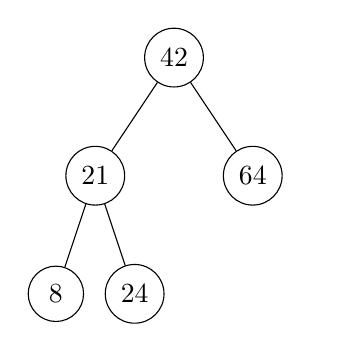
\begin{tikzpicture}[
  level/.style = {sibling distance = 20mm/#1},
  every node/.style = {minimum width = 2em, draw, circle},
  ]
  \node (n42) {42}
  child { node (n21) {21}
          child { node (n8)  {8}  }
          child { node (n24) {24} }
        }
  child { node (n64) {64}
          child { node [draw=none] (n48) {\phantom{48}} edge from parent [draw=none] }
          child { node [draw=none] (n72) {\phantom{72}} edge from parent [draw=none] }
        };
\end{tikzpicture}

  \end{minipage}
\end{table}

\vspace*{-0.5cm}

\subsubsection*{\TTBF{void print\_dfs\_inorder\_bt\_p(bt\_p *T)}}

\noindent Cette procédure exécute un \textit{parcours en profondeur} main gauche de l'arbre donné en paramètre, et affiche les clés dans l'ordre \textit{infixe}.
Chaque clé doit être suivie d'un retour à la ligne.
Si l'arbre donné en paramètre est \TTBF{NULL}, la procédure ne fait rien.

\subsubsection*{\TTBF{void print\_dfs\_postorder\_bt\_p(bt\_p *T)}}

\noindent Cette procédure exécute un \textit{parcours en profondeur} main gauche de l'arbre donné en paramètre, et affiche les clés dans l'ordre \textit{suffixe}.
Chaque clé doit être suivie d'un retour à la ligne.
Si l'arbre donné en paramètre est \TTBF{NULL}, la procédure ne fait rien.

\bigskip


\subsubsection*{\TTBF{void print\_hierarchical\_bt\_p(bt\_p *T)}}

\noindent Cette procédure exécute un \textit{parcours en largeur} de l'arbre donné en paramètre, et affiche les clés au fur et à mesure du parcours.
Chaque clé doit être suivie d'un retour à la ligne.
Si l'arbre donné en paramètre est \TTBF{NULL}, la procédure ne fait rien.

\noindent Ce qui donnerait cet affichage pour l'arbre suivant :

\begin{table}[ht!]
  \centering
  \begin{minipage}{0.45\textwidth}
    \centering

\lstset{language=sh}
\begin{lstlisting}[frame=single]
$ ./bt_example2
42
21
64
8
24
$
\end{lstlisting}

  \end{minipage}
  \hfillx
  \begin{minipage}{0.45\textwidth}
    \centering

%  level/.style = {sibling distance = 30mm/#1},
%  level 3/.style={sibling distance = 9mm},
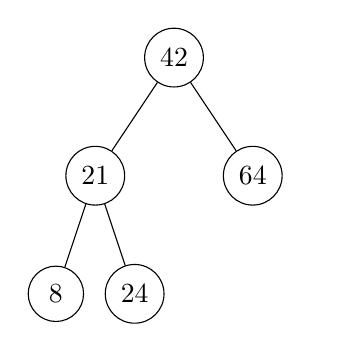
\begin{tikzpicture}[
  level/.style = {sibling distance = 20mm/#1},
  every node/.style = {minimum width = 2em, draw, circle},
  ]
  \node (n42) {42}
  child { node (n21) {21}
          child { node (n8)  {8}  }
          child { node (n24) {24} }
        }
  child { node (n64) {64}
          child { node [draw=none] (n48) {\phantom{48}} edge from parent [draw=none] }
          child { node [draw=none] (n72) {\phantom{72}} edge from parent [draw=none] }
        };
\end{tikzpicture}

  \end{minipage}
\end{table}

\vspace*{-0.5cm}

\subsubsection*{\TTBF{int hierarchical\_number\_bt\_p(bt\_p *T, int key)}}

\noindent Cette fonction récupère le numéro hiérarchique du nœud contenant la clé donnée en paramètre, puis elle le retourne.
La racine a comme numéro hiérarchique 1.
Si l'arbre donné en paramètre est \TTBF{NULL}, ou que la clé n'existe pas, la fonction doit renvoyer $ -1 $.

\bigskip


\subsubsection*{\TTBF{int clear\_bt\_p(bt\_p *T)}}

\noindent Cette fonction vide l'arbre binaire donné en paramètre en libérant chacun de ses nœuds, puis elle renvoie le nombre de nœuds libérés.
Si l'arbre donné en paramètre est \TTBF{NULL}, la fonction doit renvoyer $ 0 $.
\textit{Attention, vous ne devez pas libérer les pointeurs des éléments stockés dans les nœuds : c'est à l'utilisateur de votre bibliothèque de s'en charger.}
